\documentclass[11pt,table]{article}
\usepackage{geometry}                % See geometry.pdf to learn the layout options. There are lots.
\geometry{letterpaper}                   % ... or a4paper or a5paper or ... 
%\geometry{landscape}                % Activate for for rotated page geometry
%\usepackage[parfill]{parskip}    % Activate to begin paragraphs with an empty line rather than an indent
\usepackage{amsfonts, amscd, amssymb, amsthm, amsmath}
\usepackage{pdfsync}%leaves makers for tex searching
\usepackage{enumerate}
\usepackage{mathtools}
\usepackage{breqn}
\usepackage{tikz-cd}
\usepackage{algorithm}% http://ctan.org/pkg/algorithms
\usepackage[noend]{algpseudocode}% http://ctan.org/pkg/algorithmicx
\usepackage{xcolor}

%\usepackage{setspace} %for reducing vertical spacing in arrays
%\doublespacing

\renewcommand{\thesubsection}{\thesection.\alph{subsection}}

\usepackage{titlesec}
%\titleformat{\section}[hang]{\bfseries}{Question \thesection.\ }{0pt}{}
%\titleformat{\subsection}[hang]{\bfseries}{(\thesubsection) }{0pt}{}

%%%%% Margins %%%%% 
\setlength{\topmargin}{1in} %top/bot margins
\setlength{\oddsidemargin}{\topmargin} %sidemargins

\setlength{\textheight}{11in} \setlength{\textwidth}{8.5in}
\setlength{\hoffset}{-1in} \setlength{\voffset}{-1in} \setlength{\evensidemargin}{\oddsidemargin} \addtolength{\textheight}{-2 \topmargin}\addtolength{\textwidth}{-2\oddsidemargin}
\setlength{\headheight}{0pt} \setlength{\headsep}{20pt} \setlength{\footskip}{20pt}
\addtolength{\textheight}{-\footskip} \addtolength{\textheight}{-\headheight} \addtolength{\textheight}{-\headsep}







%%%%% Pictures %%%%% 
\usepackage{tikz}
%\usepackage{epstopdf}
%\DeclareGraphicsRule{.tif}{png}{.png}{`convert #1 `dirname #1`/`basename #1 .tif`.png}
%\usepackage[pdftex,bookmarks]{hyperref}
%
%\usepgflibrary{shapes.geometric}
%\def\ShiftX{\pgftransformxshift}
%\def\ShiftY{\pgftransformyshift}
%\tikzstyle{V}=[draw, fill =black, circle, inner sep=0pt, minimum size=2pt]
%\tikzstyle{over}=[draw=white,double=black,line width=3pt]



%% Partitions:
\newcounter{r}
\newcommand\Part[1]{
        \setcounter{r}{1}
	 \foreach \x in {#1}{
 	{\ifnum\value{r}=1
		\draw (0,\value{r}-1)--(\x,\value{r}-1); 
		\fi}
	\draw (0,\value{r}) to (\x,\value{r});
   	\foreach \y in {0, ..., \x} {\draw (\y,\value{r})--(\y,\value{r}-1);}
	\addtocounter{r}{1}
 }}
 \def\PartUNIT{.175}
%Self-contained tikz images for \Part above. 
\newcommand{\PART}[1]{
\begin{matrix}
\begin{tikzpicture}[xscale=\PartUNIT, yscale=-\PartUNIT] 
	\Part{#1}
\end{tikzpicture}
\end{matrix}
}



%%%%% Color  %%%%% 
\usepackage{color}
\definecolor{dred}{rgb}{.65, 0, 0.15}
\definecolor{violet}{rgb}{.65, 0, 0.65}
\definecolor{dgray}{rgb}{.5, .5, 0.5}
\newcommand{\NOTE}[1]{{\color{blue}#1}}
\newcommand{\DEF}[1]{{\color{violet}#1}}
\newcommand{\ASIDE}[1]{{\color{dgray}[ASIDE: #1]}}
\newcommand{\MOVED}[1]{{\color{gray}#1}}
\newcommand{\blue}[1]{{\color{blue} #1 }}


%%%%% Alphabets %%%%% 
\def\cA{\mathcal{A}}\def\cB{\mathcal{B}}\def\cC{\mathcal{C}}\def\cD{\mathcal{D}}\def\cE{\mathcal{E}}\def\cF{\mathcal{F}}\def\cG{\mathcal{G}}\def\cH{\mathcal{H}}\def\cI{\mathcal{I}}\def\cJ{\mathcal{J}}\def\cK{\mathcal{K}}\def\cL{\mathcal{L}}\def\cM{\mathcal{M}}\def\cN{\mathcal{N}}\def\cO{\mathcal{O}}\def\cP{\mathcal{P}}\def\cQ{\mathcal{Q}}\def\cR{\mathcal{R}}\def\cS{\mathcal{S}}\def\cT{\mathcal{T}}\def\cU{\mathcal{U}}\def\cV{\mathcal{V}}\def\cW{\mathcal{W}}\def\cX{\mathcal{X}}\def\cY{\mathcal{Y}}\def\cZ{\mathcal{Z}}

\def\AA{\mathbb{A}} \def\BB{\mathbb{B}} \def\CC{\mathbb{C}} \def\DD{\mathbb{D}} \def\EE{\mathbb{E}} \def\FF{\mathbb{F}} \def\GG{\mathbb{G}} \def\HH{\mathbb{H}} \def\II{\mathbb{I}} \def\JJ{\mathbb{J}} \def\KK{\mathbb{K}} \def\LL{\mathbb{L}} \def\MM{\mathbb{M}} \def\NN{\mathbb{N}} \def\OO{\mathbb{O}} \def\PP{\mathbb{P}} \def\QQ{\mathbb{Q}} \def\RR{\mathbb{R}} \def\SS{\mathbb{S}} \def\TT{\mathbb{T}} \def\UU{\mathbb{U}} \def\VV{\mathbb{V}} \def\WW{\mathbb{W}} \def\XX{\mathbb{X}} \def\YY{\mathbb{Y}} \def\ZZ{\mathbb{Z}}  

\def\fa{\mathfrak{a}} \def\fb{\mathfrak{b}} \def\fc{\mathfrak{c}} \def\fd{\mathfrak{d}} \def\fe{\mathfrak{e}} \def\ff{\mathfrak{f}} \def\fg{\mathfrak{g}} \def\fh{\mathfrak{h}} \def\fj{\mathfrak{j}} \def\fk{\mathfrak{k}} \def\fl{\mathfrak{l}} \def\fm{\mathfrak{m}} \def\fn{\mathfrak{n}} \def\fo{\mathfrak{o}} \def\fp{\mathfrak{p}} \def\fq{\mathfrak{q}} \def\fr{\mathfrak{r}} \def\fs{\mathfrak{s}} \def\ft{\mathfrak{t}} \def\fu{\mathfrak{u}} \def\fv{\mathfrak{v}} \def\fw{\mathfrak{w}} \def\fx{\mathfrak{x}} \def\fy{\mathfrak{y}} \def\fz{\mathfrak{z}}
\def\fgl{\mathfrak{gl}}  \def\fsl{\mathfrak{sl}}  \def\fso{\mathfrak{so}}  \def\fsp{\mathfrak{sp}}  
\def\GL{\mathrm{GL}} \def\SL{\mathrm{SL}}  \def\SP{\mathrm{SL}}

%shortcuts
\newcommand{\R}{\RR_{\geq 0}}
\newcommand{\ip}[2]{\left \langle #1, #2 \right \rangle}
\newcommand{\Top}{\textbf{Top}}
\newcommand{\Set}{\textbf{Set}}
\newcommand{\spec}{\text{Spec}}

%proofy
\newcommand{\ts}{\textsc{To Show: }}

%topologies
\newcommand{\topx}{\cT_X}
\newcommand{\xtop}{\left(X, \topx \right)}
\newcommand{\topy}{\cT_Y}
\newcommand{\ytop}{\left(Y, \topy \right)}

\newcommand{\ptop}{\left(\PP^1, \cT_{\PP^1}^{Zar} \right)}
\newcommand{\topp}{\cT_{\PP^1}^{Zar}}
\newcommand{\ptopstd}{\left(\PP^1, \cT_{\PP^1}^{std} \right)}
\newcommand{\toppstd}{\cT_{\PP^1}^{std}}
\newcommand{\shp}{\cO_{\PP^1}}

\newcommand{\ctop}{\left(\CC, \cT_\CC^{Zar} \right)}
\newcommand{\topc}{\cT_\CC^{Zar}}

\newcommand{\cinf}{\CC \cup \{ \infty \}}
\newcommand{\cinftop}{\left(\cinf, \cT_{\cinf} \right)}
\newcommand{\topcinf}{\cT_{\cinf}}

\newcommand{\sphtop}{\left(S^2, \cT_{S^2}^{std} \right)}
\newcommand{\topsph}{\cT_{S^2}^{std}}

\newcommand{\qtop}{\left(Q, \cT_{Q}^{Zar} \right)}
\newcommand{\topq}{\cT_{Q}^{Zar}}
\newcommand{\qtopstd}{\left(Q, \cT_{Q}^{std} \right)}
\newcommand{\topqstd}{\cT_{Q}^{std}}

%sheaves
\newcommand{\incl}[2]{\iota^{\scriptstyle #1}_{\scriptstyle #2}}
\newcommand{\resint}[3]{\mathrm{res}\begin{matrix}\scriptstyle U_{#1}\\ \scriptstyle \: U_{#2} \: \cap \: U_{#3} \end{matrix}}
\newcommand{\res}[2]{\mathrm{res} \: \begin{matrix}\scriptstyle {#1} \\ \scriptstyle {#2} \end{matrix}}

%manifolds
\newcommand{\phia}{\phi_{\alpha}}
\newcommand{\phib}{\phi_{\beta}}
\newcommand{\phiu}{\phi_{U}}
\newcommand{\phiv}{\phi_{V}}
\newcommand{\ua}{U_{\alpha}}
\newcommand{\ub}{U_{\beta}}
\newcommand{\va}{V_{\alpha}}
\newcommand{\vb}{V_{\beta}}


%%%%%%%%%%%%%%%%%%%%%%%%%%%%%% 
%%%%%%%%%%%%%%%%%%%%%%%%%%%%%%

\newcommand{\biim}{\leftrightarrow}
\newcommand{\bimv}[2]{#1\leftrightarrow{#2}}
\newcommand{\impl}{\hspace{3pt}\Rightarrow\hspace{3pt}}

\newcommand{\semR}[1]{\mathcal{S}_R(#1)}
\newcommand{\semF}[1]{\mathcal{S}_F(#1)}
\newcommand{\semFR}[1]{\mathcal{S}(#1)}
\newcommand{\ifff}{\Leftrightarrow}

\newcommand{\func}[2]{\mathbf{#1}(#2)}
\newcommand{\gap}{\hspace{4pt}}


\title{Algorithms for the GER Representation of Pos}
\author{William Price \quad 917093}
\author{Supervisors - Harald S{\o}ndergaard, Peter Schachte}
\date{March 8, 2019}                                           % Activate to display a given date or no date

\begin{document}
\maketitle


\section{Purpose}

This project provides an imperative implementation of the GER representation described by R. Bagnara and P. Schachte in \cite{bag_schachteGER}.The implementation, which we refer to as the FR representation, was developed as an extension of an existing ROBDD library written by Schachte, for use in a groundness analyser. The purpose of the F component (representing Ground and Equivalent variables) is to reduce the size of the ROBDDs by extracting redundant information. Therefore, the primary problems to solve in this project were (1) How best to represent F, and (2) how to implement the standard binary operations (and, or, implies), while preserving F information from the operands and extracting consequential F information.




\section{Definitions}
We represent a boolean function $\phi$ as a pair $ (F,R) $, where $ F $ is an equivalence relation on $ Vars \cup \left\lbrace \top, \bot \right\rbrace  $, and $ R $ is an ROBDD.

\subsection{Semantics}
\begin{itemize}
	\item $ \mathcal{S}(F,R) =  \mathcal{S}(F) \wedge  \mathcal{S}(R) $
	
	\item $\mathcal{S}_F(F) = \bigwedge \left\lbrace x \biim y | (x,y)\in F\right\rbrace $ \hspace{1in} (Note: $ x \biim \top \equiv x $, and $ x \biim \bot \equiv \neg x $)
	
	\item  $ \mathcal{S}_R(\textbf{R}) = var_R \wedge \mathcal{S}(R_{then}) \hspace{3pt} \vee \hspace{3pt} \neg var_R \wedge \mathcal{S}R_{else}$
	
	\item $ \mathcal{S}_R(\textbf{0}) = \bot $
	
	\item $ \mathcal{S}_R(\textbf{1}) = \top $
\end{itemize}

\subsection{Invariants}

To preserve the canonical form inherited from the ROBDD, we enforce the following invariants on any given $ (F,R) $ pair.

\begin{itemize}
	\item $ \forall x \in Vars: ( (\exists y\in Vars: \hspace{2pt} \hspace{2pt}(y<x) \wedge \hspace{2pt} \semFR{F,R} \vDash x\biim y) \impl x \notin dep(R))$ 
	\item[] Essentially, for any set of equivalent variables entailed by $ \semFR{F,R} $, either only the least variable in the set appears in the ROBDD, or none do. 
	\item $ \forall x\in Vars:  (\semFR{F,R}\vDash x \vee \semFR{F,R}\vDash \neg x) \impl x \notin dep(R)$
	\item $ \semF{F} \equiv \bot \ifff \semR{R} \equiv \bot $
	\item[] The following invariants are redundant, given the previous properties, however they are included for clarity.
	\item $ \forall x,y \in Vars: \semFR{F,R} \vDash x \biim y \impl (\semF{F} \vDash x\biim y \wedge \semR{R} \nvDash x\biim y)$
	\item $ \forall x \in Vars: \semFR{F,R} \vDash x \impl (\semF{F} \vDash x \wedge \semR{R} \nvDash x) $
	\item $ \forall x \in Vars: \semFR{F,R} \vDash \neg x \impl (\semF{F} \vDash \neg x \wedge \semR{R} \nvDash \neg x) $
	\item[] Lastly we must canonicalise the F-representation of $ \bot $ (The below implementation will explain how it is possible to represent a contradiction).
	\item $ \semF{F} \vDash \bot \impl \forall x,y \in Vars: (x,y) \in F $
	\item[] Therefore, the canonical representations of $ \top $ and $ \bot $ are $ (I,\textbf{1}) $ and $ (T, \textbf{0}) $, where $ I, T$ are the identity and total relations, and $ \textbf{1}, \textbf{0} $ are the true and false ROBDDs.
\end{itemize}

 

\section{F implementation}

The first structure we considered to represent F was a table representation of the relation, implemented as an array of bitsets, where bit y in bitset x is a 1-bit iff $ (x,y)\in F $ (a 0-bit otherwise). With a reasonable limit of 62 variables, this would mean an array of 64 bitsets, each 64 bits long, with table coordinates 0 and 1 reserved for $ \bot $ and $ \top $ respectively. This data structure would provide extremely logical conjunction and disjunction operations on equivalence relations, being a simple inclusive-OR or AND operation on the bits. However, this structure loses transitivity under conjunction and holds a massive amount of redundant information. For example, if \textit{w, x, y} \& \textit{z}  are all equivalent, the table tells us $ w $ is equivalent to $ x, y, z $, $ x $ is equivalent to $ w,y,z $, $ y $ is equivalent to $ w,x,z $ \textit{etc}. 

\subsection{Union-Find F-Equivalence}

Noting transitivity as a priority, we instead opted for a union-find data structure. F is represented as an array of variables, where $ F[x]=y $ iff $ \left(x\leq y \textbf{ and } (x,y)\in F \right)$. In this situation, $ y $ is considered the $ parent $ of $ x $, being a smaller-equivalent variable (so $ parent(x)=F[x]$). Again we reserve 0 and 1 as variable indexes for $ \bot $ and $ \top $ respectively, but will refer to them by name below for clarity (instead of index). The least-equivalent variable we call the $ root $ of $ x $, and can be found through repeated iteration of array indexing ($ F[F[F[....F[x]]]] $), until a fixed point is reached (the parent of a root is itself). This data structure can be visualised as clustered DAGs, where each cluster is an equivalence class, and the sink node in each cluster is the root variable node of that equivalence class.

\begin{figure}[h]
	\caption{An example F-equivalence}
	\centering
	
	\vspace{0.3in}
	\begin{tabular}{|c|c|c|c|c|c|c|c|c|c|}
		\hline
		$ x $        & $\bot$ & $\top$ & 2 & 3 & 4 & 5 & 6 & 7 & 8 \\ \hline
		$ F[x] $ & $\bot$ & $\top$ & 2 & 3 & 2 & 3 & 3 & 6 & 2 \\ \hline
	\end{tabular}
	\vspace{0.3in}

	\begin{tikzpicture}[scale=0.2]
	\tikzstyle{every node}+=[inner sep=0pt]
	\draw [black] (32,-24.1) circle (3);
	\draw (32,-24.1) node {$2$};
	\draw [black] (28,-36.2) circle (3);
	\draw (28,-36.2) node {$4$};
	\draw [black] (35.6,-36.2) circle (3);
	\draw (35.6,-36.2) node {$8$};
	\draw [black] (48.7,-24.1) circle (3);
	\draw (48.7,-24.1) node {$3$};
	\draw [black] (45,-33.4) circle (3);
	\draw (45,-33.4) node {$5$};
	\draw [black] (52.7,-33.4) circle (3);
	\draw (52.7,-33.4) node {$6$};
	\draw [black] (48.7,-40.7) circle (3);
	\draw (48.7,-40.7) node {$7$};
	\draw [black] (18.4,-36.2) circle (3);
	\draw (18.4,-36.2) node {$\top$};
	\draw [black] (18.4,-24.1) circle (3);
	\draw (18.4,-24.1) node {$\bot$};
	\draw [black] (28.94,-33.35) -- (31.06,-26.95);
	\fill [black] (31.06,-26.95) -- (30.33,-27.55) -- (31.28,-27.86);
	\draw [black] (34.74,-33.32) -- (32.86,-26.98);
	\fill [black] (32.86,-26.98) -- (32.6,-27.88) -- (33.56,-27.6);
	\draw [black] (46.11,-30.61) -- (47.59,-26.89);
	\fill [black] (47.59,-26.89) -- (46.83,-27.45) -- (47.76,-27.82);
	\draw [black] (50.14,-38.07) -- (51.26,-36.03);
	\fill [black] (51.26,-36.03) -- (50.44,-36.49) -- (51.31,-36.97);
	\draw [black] (51.51,-30.64) -- (49.89,-26.86);
	\fill [black] (49.89,-26.86) -- (49.74,-27.79) -- (50.66,-27.39);
	\draw [black] (30.677,-21.42) arc (234:-54:2.25);
	\fill [black] (33.32,-21.42) -- (34.2,-21.07) -- (33.39,-20.48);
	\draw [black] (47.377,-21.42) arc (234:-54:2.25);
	\fill [black] (50.02,-21.42) -- (50.9,-21.07) -- (50.09,-20.48);
	\draw [black] (17.077,-33.52) arc (234:-54:2.25);
	\fill [black] (19.72,-33.52) -- (20.6,-33.17) -- (19.79,-32.58);
	\draw [black] (17.077,-21.42) arc (234:-54:2.25);
	\fill [black] (19.72,-21.42) -- (20.6,-21.07) -- (19.79,-20.48);
	\end{tikzpicture}
\end{figure}

Two variables $ x $ and $ y $ are therefore equivalent iff $ \textbf{root}(x)=\textbf{root}(y) $. To ensure that any equivalence class does not have more than one root (sink) node, we implement the union algorithm so that the roots of the inputs are linked, rather than the inputs themselves.


\begin{algorithm}
	\begin{algorithmic}[1]
		\Function{union-simple}{$a,b$}
		
		\If{$ \textbf{root}(a) < \textbf{root}(b) $}
		\State $ F[\textbf{root}(b)] \gets \textbf{root}(a)) $
		
		\ElsIf{$ \textbf{root}(a) > \textbf{root}(b) $}
		\State $ F[\textbf{root}(a)] \gets \textbf{root}(b)) $
		\EndIf
		
		\EndFunction
	\end{algorithmic}
\end{algorithm}

The use of this function for unifying variables gives us transitivity for free, as we can check equivalence of variables by checking if $ \textbf{root}(a) = \textbf{root}(b)$. The condition that ensures the larger root is parented by the smaller root imposes a strict ordering on the variables along any path to the root node, such that the root of any variable is always the least variable in it's entire equivalence class. This is valuable, as it allows us to pick a canonical representative of each equivalence class for use in the ROBDD.

This data structure functions correctly using only the union algorithm (and its primitive root algorithm) , however, unifying many variables in descending order can lead to long chains of variables, which leaves our test for equivalence algorithm at $ O(n) $ time to find the roots and compare. To avoid this, we would like to link child nodes directly to their roots wherever possible, therefore shortening the path from any grandchild-nodes. This is done during the root-finding algorithm, $ \textbf{find}(x) $, which, after following a path from a child node to the root-node, recursively links every node along that path directly to the root.

\begin{algorithm}
	%	\caption{Euclid’s algorithm}\label{euclid}
	\begin{algorithmic}[1]
		\Function{find}{$x$}
		
		\If{$ F[F[x]] \neq F[x]  $} \Comment{Check if $ x $'s parent isn't a root}
		\State $ F[F[x]] \gets $ {\Call{find}{$F[x]$}} \Comment{Link $ x $'s parent directly to the root}
		
		\EndIf
		
		\State $ F[x] = F[F[x]] $
		\State \textbf{return} $ F[x] $
		
		\EndFunction
	\end{algorithmic}
\end{algorithm}

We update the \textbf{union} algorithm to use \textbf{find}. Employing \textbf{find} every time a root is needed amortises the look-up cost, but we still have a worst case complexity of $ O(n) $, in the case where many variables are linked in descending order. Other implementations of this structure will often compare the \textit{rank/size} of the roots to ensure the root of the smaller group of nodes is pointed to the root of the larger, keeping the majority of paths short. This metric gives an amortised constant time \textbf{find} operation, however, we would then have to scan the array in linear time to determine the correct least-equivalent variable.

\begin{algorithm}
	\begin{algorithmic}[1]
		\Function{union}{$a,b$}
		\State $ a\_root, b\_root \gets $ \Call{find}{$a$}, \Call{find}{$b$}
		
		\If{$ a\_root < b\_root $}
			\State $ F[b\_root] \gets a\_root $
		\ElsIf{$ a\_root > b\_root $}
			\State $ F[a\_root] \gets b\_root $
		\EndIf
		
		\EndFunction
	\end{algorithmic}
\end{algorithm}

\begin{figure}[h]
	\caption{The result of calling \textbf{union}(7,8) on the equivalence from Fig 1.}
	\centering
	
	\vspace{0.3in}
	\begin{tabular}{|c|c|c|c|c|c|c|c|c|c|}
		\hline
		$ x $        & $ \bot $ & $ \top $ & 2 & 3 & 4 & 5 & 6 & 7 & 8 \\ \hline
		$ F[x] $    & $ \bot $ & $ \top $ & 2 & 2 & 2 & 3 & 3 & 3 & 2 \\ \hline
	\end{tabular}
	\vspace{0.3in}
	
	\begin{tikzpicture}[scale=0.2]
	\tikzstyle{every node}+=[inner sep=0pt]
	\draw [black] (32.2,-24.1) circle (3);
	\draw (32.2,-24.1) node {$2$};
	\draw [black] (28,-36.2) circle (3);
	\draw (28,-36.2) node {$4$};
	\draw [black] (35.6,-36.2) circle (3);
	\draw (35.6,-36.2) node {$8$};
	\draw [black] (48.7,-24.1) circle (3);
	\draw (48.7,-24.1) node {$3$};
	\draw [black] (44.8,-36.2) circle (3);
	\draw (44.8,-36.2) node {$5$};
	\draw [black] (52.4,-36.2) circle (3);
	\draw (52.4,-36.2) node {$6$};
	\draw [black] (60.6,-36.2) circle (3);
	\draw (60.6,-36.2) node {$7$};
	\draw [black] (18.4,-36.2) circle (3);
	\draw (18.4,-36.2) node {$\top$};
	\draw [black] (18.4,-24.1) circle (3);
	\draw (18.4,-24.1) node {$\bot$};
	\draw [black] (28.98,-33.37) -- (31.22,-26.93);
	\fill [black] (31.22,-26.93) -- (30.48,-27.53) -- (31.43,-27.85);
	\draw [black] (34.79,-33.31) -- (33.01,-26.99);
	\fill [black] (33.01,-26.99) -- (32.75,-27.89) -- (33.71,-27.62);
	\draw [black] (45.72,-33.34) -- (47.78,-26.96);
	\fill [black] (47.78,-26.96) -- (47.06,-27.56) -- (48.01,-27.87);
	\draw [black] (51.52,-33.33) -- (49.58,-26.97);
	\fill [black] (49.58,-26.97) -- (49.33,-27.88) -- (50.29,-27.59);
	\draw [black] (30.877,-21.42) arc (234:-54:2.25);
	\fill [black] (33.52,-21.42) -- (34.4,-21.07) -- (33.59,-20.48);
	\draw [black] (17.077,-33.52) arc (234:-54:2.25);
	\fill [black] (19.72,-33.52) -- (20.6,-33.17) -- (19.79,-32.58);
	\draw [black] (17.077,-21.42) arc (234:-54:2.25);
	\fill [black] (19.72,-21.42) -- (20.6,-21.07) -- (19.79,-20.48);
	\draw [black] (45.7,-24.1) -- (35.2,-24.1);
	\fill [black] (35.2,-24.1) -- (36,-24.6) -- (36,-23.6);
	\draw [black] (58.5,-34.06) -- (50.8,-26.24);
	\fill [black] (50.8,-26.24) -- (51.01,-27.16) -- (51.72,-26.46);
	\end{tikzpicture}
\end{figure}



The following functions naturally arises from \textbf{union} and \textbf{find}.
\begin{itemize}
	\item $ \func{entail}{x} := \func{union}{\top,x} $
	\item $ \func{disentail}{x} := \func{union}{\bot,x} $
	\item $ \func{are\_equivalent}{x,y} := (\func{find}{x}=\func{find}{y}) $
	\item $ \func{is\_entailed}{x} := (\func{find}{x}=\top) $
	\item $ \func{is\_disentailed}{x} := (\func{find}{x}=\bot) $
\end{itemize}

Lastly, we redefine $ \mathcal{S}_F $ such that if $ \func{is\_disentailed}{\top} $ is true, then $ \semF{F} = \bot $. This happens if either $ \func{entail}{x} $ is called where $ \func{is\_disentailed}{x} $ is true, or $ \func{disentail}{x} $ is called where $  \func{is\_entailed}{x} $ is true. In terms of the actual code, we use a special pointer value for the false-equivalence, to which any equivalence is converted as soon as a contradiction occurs. This avoids the need to write the total equivalence to the entire array (as specified under the invariances), and allows the false-equivalence to be recognised and passed efficiently.

\subsection{Equivalence operations}

In order to perform logical operations on $ (F,R) $ pairs, we must first define them on Equivalences.

\subsubsection{equiv\_and}
The logical AND of two equivalences, F, G, is the transitive closure of their union.  For example (ignoring symmetry) if $ \bimv{x}{y} \in F $ and $ \bimv{y}{z} \in G $, then $ \bimv{x}{y}, \bimv{y}{z}, \bimv{x}{z} $ should all be in $ \func{equiv\_and}{F,G} $.

To simplify the access of root variables, we first apply the algorithm \textbf{flatten} to both F and G.

\begin{algorithm}
	\begin{algorithmic}[1]
		\Function{flatten}{$ F $}
		
		\For{$ x $ in $ Vars $}
		\State $ find(x) $
		\EndFor
		
		\EndFunction
	\end{algorithmic}
\end{algorithm}

To perform the union, we allocate a new Equivalence $ H $ to write the result, and proceed in ascending order along the F and G arrays in parallel. For each variable index $ x $, we inspect it's root in $ F $, $ \func{root_F}{x} $ and its root in G, $ \func{root_G}{x} $ (remember these are just $ F[x] $ and $ G[x] $ because of the \textbf{flatten} calls). If $ \func{root_F}{x} $ and $ \func{root_G}{x} $ are different, we have 3 different variables we must unify. Writing either of these roots of x at $ H[x] $ will lose the connection to the other, so we must first unify the roots in $ H $. This means simply finding the smaller of the roots of the $ F $ and $ G $ roots in $ H $, i.e. $ common\_root = \func{min}{H[\func{root_F}{x}], H[\func{root_F}{x}]} $. This will always be defined, because $ \func{root_F}{x} $ and $ \func{root_G}{x} $ must both be smaller than $ x $ and we have already assigned parents for every variable up to $ x $ in $ H $. We now set $ H[\func{root_F}{x}], H[\func{root_F}{x}] $ and $ H[x] $ all equal to $ common\_root $, and we have the unification. Now any variable linked to $ \func{root_F}{x} $ or $ \func{root_G}{x} $ in either $ F $ or $ G $ will be transitively linked to $ common\_root $. For the case where $ \func{root_F}{x} $ $ \func{root_G}{x} $, we can actually use this same process, as we are essentially just writing $ H[F[x]] $ to $ H[x] $ instead of just $ F[x]] $, which points $ x $ directly to its root, rather than going through $ F[x] $. 
One extra step 
The below algorithm is presented in simple form, but can be easily expanded to reduce the amount of redundant writing.

\begin{algorithm}
	\begin{algorithmic}[1]
		\Function{equiv\_and}{$ F,G $}
		\State \Call{allocate\_equiv}{$ H $} 
		\For{$ x $ in $ Vars $}
		\State $ H[x], \gap H[F[x]], \gap H[G[x]] \gets \func{min}{H[F[x]], \gap H[G[x]]}$
		\EndFor
		
		\EndFunction
	\end{algorithmic}
\end{algorithm}

\subsubsection{equiv\_or}

The logical OR of two equivalences is a bit more complicated, as we must only retain the variable equivalences found in both $ F $ and $ G $. The complication arises in the fact that 2 variables can share an equivalence class in both $ F $ and $ G $, but those classes need not have the same root variable. Therefore we cannot just intersect roots.

The below is a clear example of what should happen. 4 and 7 are linked to each-other in both Equivalences, however in $ F $ their root is $ 2 $, and in $ G $ it's 3. 

\begin{figure}[h]
	\centering
	\begin{tabular}{|c|c|c|c|c|l|l|}
		\hline
		$x$              & 2                           		& 3                                 & 4                         & 5                         & 6                         & 7                         \\ \hline
		$F[x]$          & \cellcolor{red!25}2	  & \cellcolor{yellow!25}3   & \cellcolor{green!25}2 & \cellcolor{yellow!25}3 & \cellcolor{blue!25}3 & \cellcolor{green!25}2 \\ \hline
		$G[x]$         & \cellcolor{red!25}2      & \cellcolor{yellow!25}3  & \cellcolor{green!25}3 & \cellcolor{yellow!25}3 & \cellcolor{blue!25}2 & \cellcolor{green!25}3 \\ \hline
		$(F\vee G)[x]$ & \cellcolor{red!25}2  & \cellcolor{yellow!25}3   & \cellcolor{green!25}4 & \cellcolor{yellow!25}3 & \cellcolor{blue!25}6 & \cellcolor{green!25}4 \\ \hline
	\end{tabular}
	\vspace{.2in}

	\begin{tikzpicture}[scale=0.2]
	\tikzstyle{every node}+=[inner sep=0pt]
	\draw [black] (17.7,-19.6) circle (3);
	\draw (17.7,-19.6) node {$2$};
	\draw [black] (14,-27.8) circle (3);
	\draw (14,-27.8) node {$4$};
	\draw [black] (20.9,-27.8) circle (3);
	\draw (20.9,-27.8) node {$7$};
	\draw [black] (31.8,-40.3) circle (3);
	\draw (31.8,-40.3) node {$3$};
	\draw [black] (25.2,-47.9) circle (3);
	\draw (25.2,-47.9) node {$4$};
	\draw [black] (31.8,-47.9) circle (3);
	\draw (31.8,-47.9) node {$5$};
	\draw [black] (31.8,-19.6) circle (3);
	\draw (31.8,-19.6) node {$3$};
	\draw [black] (17.7,-39.7) circle (3);
	\draw (17.7,-39.7) node {$2$};
	\draw [green!66, ultra thick] (63,-32) circle (3);
	\draw (63,-32) node {$4$};
	\draw [green!66, ultra thick] (63,-40.3) circle (3);
	\draw (63,-40.3) node {$7$};
	%\draw [black] (25.2,-15) circle (3);
	\draw (25.2,-15) node {$\mathbf{F}$};
	%\draw [black] (25.2,-38.3) circle (3);
	\draw (25.2,-35.3) node {$\mathbf{G}$};
	\draw [red!66, ultra thick] (47.7,-32) circle (3);
	\draw (47.7,-32) node {$2$};
	\draw [yellow!66, ultra thick] (55.5,-32) circle (3);
	\draw [black] (55.5,-32) circle (3);
	\draw (55.5,-32) node {$3$};
	%\draw [black] (59.3,-23.6) circle (3);
	\draw (59.3,-23.6) node {$\mathbf{F\vee G}$};
	\draw [black] (36.3,-27.8) circle (3);
	\draw (36.3,-27.8) node {$6$};
	\draw [black] (28.7,-27.8) circle (3);
	\draw (28.7,-27.8) node {$5$};
	\draw [black] (38.8,-47.9) circle (3);
	\draw (38.8,-47.9) node {$7$};
	\draw [black] (17.7,-47.9) circle (3);
	\draw (17.7,-47.9) node {$6$};
	\draw [yellow!66, ultra thick] (55.5,-40.3) circle (3);
	\draw [black!66] (55.5,-40.3) circle (3);
	\draw (55.5,-40.3) node {$5$};
	\draw [blue!66, ultra thick] (70.3,-32) circle (3);
	\draw (70.3,-32) node {$6$};
	\draw [black] (15.23,-25.07) -- (16.47,-22.33);
	\fill [black] (16.47,-22.33) -- (15.68,-22.86) -- (16.59,-23.27);
	\draw [black] (19.81,-25.01) -- (18.79,-22.39);
	\fill [black] (18.79,-22.39) -- (18.62,-23.32) -- (19.55,-22.96);
	\draw [black] (27.17,-45.63) -- (29.83,-42.57);
	\fill [black] (29.83,-42.57) -- (28.93,-42.84) -- (29.69,-43.5);
	\draw [black] (31.8,-44.9) -- (31.8,-43.3);
	\fill [black] (31.8,-43.3) -- (31.3,-44.1) -- (32.3,-44.1);
	\draw [black] (16.377,-16.92) arc (234:-54:2.25);
	\fill [black] (19.02,-16.92) -- (19.9,-16.57) -- (19.09,-15.98);
	\draw [black] (30.477,-37.62) arc (234:-54:2.25);
	\fill [black] (33.12,-37.62) -- (34,-37.27) -- (33.19,-36.68);
	\draw [black] (30.477,-16.92) arc (234:-54:2.25);
	\fill [black] (33.12,-16.92) -- (34,-16.57) -- (33.19,-15.98);
	\draw [black] (16.377,-37.02) arc (234:-54:2.25);
	\fill [black] (19.02,-37.02) -- (19.9,-36.67) -- (19.09,-36.08);
	\draw [black] (63,-37.3) -- (63,-35);
	\fill [black] (63,-35) -- (62.5,-35.8) -- (63.5,-35.8);
	\draw [black] (61.677,-29.32) arc (234:-54:2.25);
	\fill [black] (64.32,-29.32) -- (65.2,-28.97) -- (64.39,-28.38);
	\draw [black] (46.377,-29.32) arc (234:-54:2.25);
	\fill [black] (49.02,-29.32) -- (49.9,-28.97) -- (49.09,-28.38);
	\draw [black] (54.177,-29.32) arc (234:-54:2.25);
	\fill [black] (56.82,-29.32) -- (57.7,-28.97) -- (56.89,-28.38);
	\draw [black] (34.86,-25.17) -- (33.24,-22.23);
	\fill [black] (33.24,-22.23) -- (33.19,-23.17) -- (34.07,-22.69);
	\draw [black] (29.76,-24.99) -- (30.74,-22.41);
	\fill [black] (30.74,-22.41) -- (29.99,-22.98) -- (30.92,-23.33);
	\draw [black] (36.77,-45.69) -- (33.83,-42.51);
	\fill [black] (33.83,-42.51) -- (34.01,-43.43) -- (34.74,-42.76);
	\draw [black] (17.7,-44.9) -- (17.7,-42.7);
	\fill [black] (17.7,-42.7) -- (17.2,-43.5) -- (18.2,-43.5);
	\draw [black] (55.5,-37.3) -- (55.5,-35);
	\fill [black] (55.5,-35) -- (55,-35.8) -- (56,-35.8);
	\draw [black] (68.977,-29.32) arc (234:-54:2.25);
	\fill [black] (71.62,-29.32) -- (72.5,-28.97) -- (71.69,-28.38);
	\end{tikzpicture}
\end{figure}

So how do we recognise this situation? Firstly we apply \textbf{flatten} to both $ F $ and $ G $ so we can see the roots directly. Now if we look each $ (\func{root_F}{x}, \func{root_G}{x}) $ as an ordered pair, we can recognise the unique signature of each equivalence class resulting from the intersection of $ F $ and $ G $. The job of the algorithm is to find the least variable for each signature, and write that as the root of all other variables with the same signature. This can be done in $ O(n^2) $ time by looking back through the array every time to find the least variable with the same signature, but we can do better by using a hash table. For each $ x $ in $ Vars $ (ascending), we check the hash table for a stored root-value at $ (\func{root_F}{x}, \func{root_G}{x}) $, writing it at $ H[x] $ if it exists. Otherwise this is the first variable with signature $ (\func{root_F}{x}, \func{root_G}{x}) $, and must be the root of any later variables with the same signature. Therefore we store $ x $ at key $ (\func{root_F}{x}, \func{root_G}{x}) $ in the hash-table and write $ x $ at $ H[x] $.

\begin{algorithm}
	\begin{algorithmic}[1]
		\Function{equiv\_or}{$ F,G $}
		\State \Call{allocate\_equiv}{$ H $} 
		\State \Call{init\_hash\_table}{T}
		\For{$ x $ in $ Vars $}
		\If{$ T\left[F\left[x\right]\right]\left[G\left[x\right]\right] $ is valid variable}
			\State $ H[x] \gets T\left[F\left[x\right]\right]\left[G\left[x\right]\right]  $
		\Else
			\State $ H[x] \gets x$
			\State $ T\left[F\left[x\right]\right]\left[G\left[x\right]\right]  \gets x $
		\EndIf
		\EndFor
		
		\EndFunction
	\end{algorithmic}
\end{algorithm}


\section{Canonicalisation}

Before we can implement binary operations on $ (F,R) $ pairs, we need algorithms for canonicalisation to ensure that the invariant properties described in section 2.b hold.

We define two similar functions: $ \func{canon\_ROBDD}{R} $ and $ \func{canon\_wrt}{F,R} $.

\subsection{canon\_ROBDD}

This function takes any ROBDD, R, and returns a canonicalised pair $ (F,R') $, such that $ \semFR{F,R'} \equiv \semR{R} $.
There are two stages for this function. We first extract all equivalent, entailed and disentailed variables from the ROBDD storing them in the new $ F $ component of the returned pair, then we minimise the ROBDD with respect to the equivalent variables in $ F $, leaving only root variables in the ROBDD (if necessary).

\begin{algorithm}
	\begin{algorithmic}[1]
		\Function{canon\_ROBDD}{$ R $}
		\If{\Call{is\_terminal}{$ R $}}
			\If{$ R = \mathbf{0} $}
				\Return (\Call{false\_equivalence}{}, \textbf{0})
			\Else{}
				\Return (\Call{true\_equivalence}{}, \textbf{1})
			\EndIf
		\Else	
		
			\State $ F \gets  $ \Call{extract\_equivs}{$ R $}
			
			\State $ R' \gets $ \Call{self\_minimise}{$ F,R $}
			
			\State \Return $ (F,R') $

		\EndIf
		\EndFunction
	\end{algorithmic}
\end{algorithm}


\subsubsection{extract\_equivs}

As is natural for any ROBDD algorithm, we extract the Equivalences recursively. For terminal nodes, we return the appropriate trivial Equivalence. For non-terminal nodes, $ R $, we check if either child node is the terminal \textbf{0}-node. This either entails or disentails $ R_{var} $, so we recursively retrieve the equivalences found on the non-zero child-node and add the relevant entailment/disentailment of $ R_{var} $. Otherwise we can neither say $ R_{var} $ is definitely true or definitely false. In this case, we intend to intersect the equivalences found on $ R_{then} $ and $ R_{else} $ (those variables that are equivalent regardless of $ R_{var} $'s value). Not only this, we also need to recognise variables that are entailed when $ R_{var} $ is true and disentailed when $ R_{var} $ is false (these variables are logically equivalent to $ R_{var} $). Both of these jobs are handled by $ \func{equiv\_then\_or\_else}{R, then, else} $, which identical to $ \func{equiv\_or}{F,G} $, except when the signature $ (\func{root_{then}}{x}, \func{root_{else}}{x}) $ is $ (\top, \bot) $, it writes $ R_{var} $.

\begin{algorithm}
	\begin{algorithmic}[1]
		\Function{extract\_equivs}{$ R$}
		\If{\Call{is\_terminal}{$ R $}}
			\If{$ R = \mathbf{0} $}
				\Return \Call{identity\_equivalence}{}
			\ElsIf{$ R = \mathbf{1} $}
				\Return \Call{false\_equivalence}{}
			\EndIf
		\Else
			
			\If{$ R_{else} = \mathbf{0} $ }
				\State $ result \gets  $ \Call{extract\_equivs}{$ R_{then} $}
				\State $ result.\func{entail}{R_{var}} $
				\State \Return $ result $
			\ElsIf{$ R_{then} = \mathbf{0} $}
				\State $ result \gets $ \Call{extract\_equivs}{$ R_{else} $}
				\State $ result.\func{disentail}{R_{var}} $
				\State \Return $ result $
			\Else
				\State $ equiv\_then \gets $ \Call{extract\_equivs}{$ R_{then} $}
				\State $ equiv\_else \hspace{3.5pt} \gets $ \Call{extract\_equivs}{$ R_{else} $}
				\State \Return \Call{equiv\_then\_or\_else}{$ R, equiv\_then, equiv\_else $}
			\EndIf
		\EndIf
		
		\EndFunction
	\end{algorithmic}
\end{algorithm}

\subsubsection{self\_minimise}

After extracting the equivalences into the $ F $-structure, we need to remove them from the ROBDD to enforce the invariant property that only $ F $ store this information. $ \func{minimise}{F,R} $ does this job recursively, returning the most ``reduced'' ROBDD, $ R' $, such that $ \semFR{F,R} \equiv \semFR{F,R'}$. For example, if $ \semR{R} \equiv w \wedge (\bimv{x}{y}) \wedge (y \vee z) $, then $ F = \func{extract\_equivs}{R} $ would be semantically $ w \wedge \bimv{x}{y} $. After calling $ R' = \func{minimise}{F,R}  $, we want $ R' $ to simply represent $ x \vee z $. This is because, both $ w $ and $ \bimv{x}{y} $ are already represented by $ F $, and to keep it canonical, we need to have the ROBDD represent $ x \vee z $ rather than $ y \vee z$, as $ x $ is the least variable equivalent to $ y $.

Since the equivalence information is still present in ROBDD, we can easily remove entailed, disentailed, or non-root-variables by restricting those variables to the appropriate boolean value. While executing, if the current node is non-terminal and either entailed or disentailed in $ F $ then one of it's children must be the zero-node, so we simply replace it with the non-zero child. We do the same thing when we find a node, $ R $, where $ R_{var} \neq F.\func{find}{R_{var}}$, as a choice must have been made for $ R_{var} $'s root-variable along the path to this node, meaning one of children of $ R $ must be the zero-node. For all other non-terminal nodes, $ R $, which are root-variables of their equivalence classes (possibly singleton sets), we simply minimise both children nodes, then reconstruct the node with \textbf{make\_node} to preserve the reduced nature of the ROBDD.

Note this algorithm is equivalent to performing existential quantification over every non-root variable in the Equivalence (see the \textit{projection} algorithms in \cite{bag_schachteR}).

\begin{algorithm}
	\begin{algorithmic}[1]
		\Function{self\_minimise}{$ F,R $}
			\If{\Call{is\_terminal}{$ R $}}
			\Return $ R $
			\Else
				\State $ root\_var \gets F.\func{find}{R_{var}}$
				\State
				\If{$ root\_var \neq R_{var} $}
					\If{$ R_{else} = \mathbf{0}  $}
						\Return \Call{self\_minimise}{$ R_{then} $}
					\Else{}
						\Return \Call{self\_minimise}{$ R_{else} $}
					\EndIf
					\State
				\Else
					\State \Return $ \func{make\_node}{ R_{var} , \Call{minimise\_aux}{ F,R_{then}}, , \Call{minimise\_aux}{F,R_{else}}} $
				\EndIf
			\EndIf
		\EndFunction
	\end{algorithmic}
\end{algorithm}



\begin{algorithm}
	\begin{algorithmic}[1]
		\Function{minimise\_wrt}{$ F,R $}
			\State $ entailed[] \gets  $ \Call{init\_zeroes}{ }
			\State $ disentailed[] \gets  $ \Call{init\_zeroes}{ }
			\State \Return \Call{minimise\_aux}{$ F,R,entailed,disentailed $}
			\State 
		\EndFunction
		\Function{minimise\_aux}{$ F,R,entailed[],disentailed[] $}
		\If{\Call{is\_terminal}{$ R $}}
			\Return $ R $
		\Else
			\State $ root\_var \gets F.\func{find}{R_{var}}$
			\State
			\If{$ root\_var = \top $ or $ entailed[root\_var] = \mathbf{true} $}
				\State \Return \Call{minimise\_aux}{$ F,R_{then}, entailed, disentailed $}
				\State
			\ElsIf{$ root\_var = \bot $ or $ disentailed[root\_var] = \mathbf{true} $}
				\State \Return \Call{minimise\_aux}{$ F,R_{else}, entailed, disentailed $}
			\Else
			\State
			\State $ entailed[root\_var]  = \mathbf{true} $
			\State $ new\_then \gets $ \Call{minimise\_aux}{$ F,R_{then}, entailed, disentailed $}
			\State $ entailed[root\_var]  = \mathbf{false} $
			\State
			\State $ disentailed[root\_var]  = \mathbf{true} $
			\State $ new\_else \gets $ \Call{minimise\_aux}{$ F,R_{else}, entailed, disentailed $}
			\State $ entailed[root\_var]  = \mathbf{false} $
			\State
			
			\State \Return \Call{make\_node}{$ R_{var}, new\_then, new\_else $}
			\EndIf
			
		\EndIf
			
		\EndFunction
	\end{algorithmic}
\end{algorithm}


\begin{thebibliography}{9}

\bibitem{bag_schachteGER}
	R. Bagnara and P. Schachte. Efficient Implementations of \textit{Pos}

\bibitem{bag_schachteR}
	R. Bagnara and P. Schachte. Factorizing Equivalent Variable Pairs in ROBDD-Based Implementations of \textit{Pos}.
  
\end{thebibliography}

\end{document}  